\chapter{Casos de uso}
\section{Diagrama}
\newpage
\begin{figure}[H]
\centering
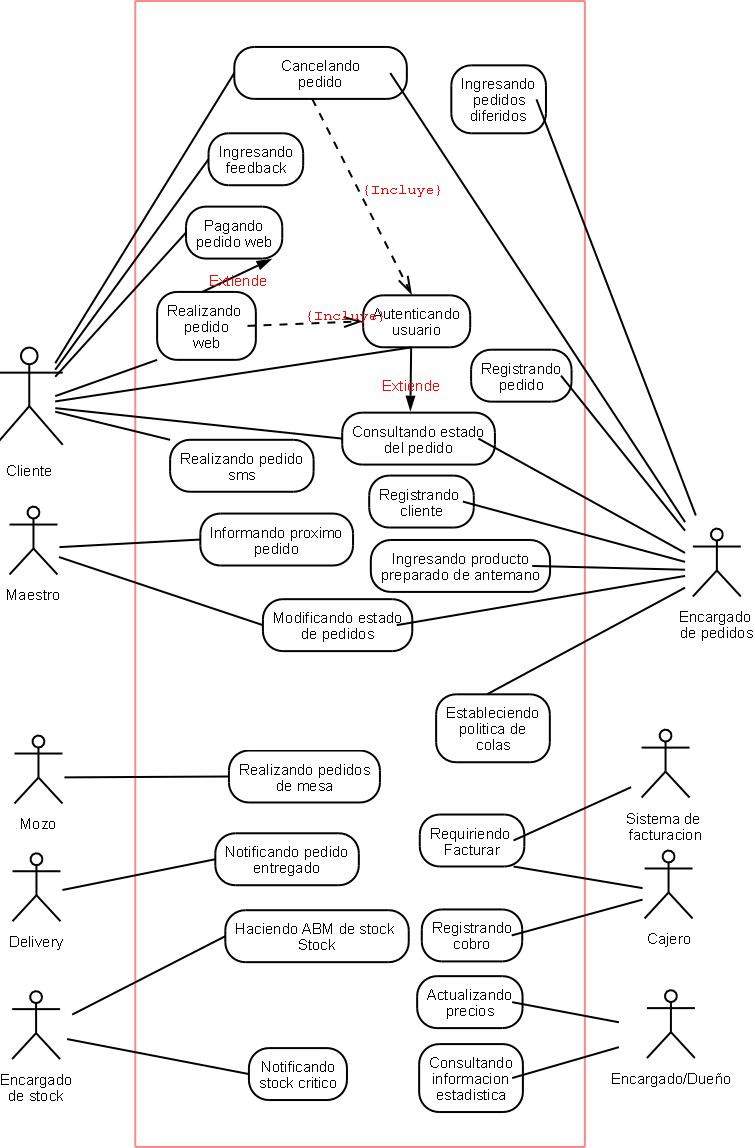
\includegraphics[scale=0.35]{casosdeuso.png}
\end{figure}

\section{Breve descripci�n}
A continuacion daremos a modo ilustrativo una breve descripci�n de los casos de uso 
considerados en el diagrama. La misma no pretende ser exahustiva, sino simplemente presentar 
un panorama de a que se refiere cada caso de uso.

\setcounter{subsection}{0}
\subsection{Autenticando usuario}

\textit{Agente: Cliente}

Para poder acceder a los distintos servicios via web que ofrece la pizzer�a, es necesario 
que el usuario se identifique. Para obtener una cuenta de usuario, el mismo tuvo que 
registrarse ya sea personal o telefonicamente.

Este caso de uso esta relacionado con el objetivo de lograr ampliar la forma de registro de 
pedidos, asi como tambi�n ayuda a poder lograr que los usuarios cancelen pedidos, consulten 
el estado de los mismo y lo paguen via internet.

\subsection{Realizando pedido via web}

\textit{Agente: Cliente}

El usuario, una vez autenticado, puede armar un pedido a traves de la pagina web de la 
pizzer�a. Una vez elegidos los productos que desea pedir, podr� optar por pagarlo en 
efectivo al delivery o pagar a traves de tarjeta de credito. Ademas el sistema le dar� alg�n 
identificador de pedido que le permita consultar el estado del mismo. Si el pedido no se 
puede armar, porque no hay productos para hacerlo, el sistema muestra un mensaje al usuario.

Este caso de uso sirve para poder lograr ampliar la forma de hacer pedidos por parte de los 
clientes.

\subsection{Pagando via web}

\textit{Agente: Cliente}

El usuario, al realizar un pedido puede elegir hacer un pago via web utilizando la tarjeta 
de credito.

Este caso de uso es tambi�n necesario para poder lograr que los usuarios hagan pedidos de 
varias formas

\subsection{Cancelando pedido} % TODO: hasta cuando puede cancelar? Que objetivos cumple

\textit{Agentes: Cliente, encargado de pedidos}

Este caso de uso permite que en cualquier momento el usuario pueda cancelar un pedido que 
realizo. Para poder hacerlo debe loguearse en el sistema y utilizar el identificador de 
pedido que se le brindo al momento de realizar el pedido. Ademas el cliente podria 
comunicarse telefonicamente, de modo que el encargado de pedidos es el que realiza la 
cancelacion del pedido.

Este caso de uso es util para permitir que los usuarios tengan una interaccion mas fluida 
con la pizzeria.

\subsection{Realizando pedido via sms}

\textit{Agente: Cliente}

Como alternativa al pedido telefonico, web o personal, es posible hacer un pedido mediante 
sms, para esto el usuario tiene que haberse registrado anteriormente. Para hacerlo, se utilizan codigos que permiten identificar que quiere el usuario. Si no se puede hacer el pedido, se enviara un mensaje al usuario notificandolo de la situaci�n.

Este caso de uso ayuda a lograr nuevas formas de registrar pedidos por parte de los usuarios.

\subsection{Ingresando feedback}

\textit{Agente: Cliente}

Una vez realizada la entrega de un pedido por delivery, el usuario tiene la posibilidad de 
opinar sobre el servicio mediante internet. Para esto es necesario que el usuario se logue.

Esta informaci�n u opiniones sobre el servicio ayudan a lograr informaci�n estadistica sobre 
el funcionamiento de la pizzeria, la cual podria usarse para identificar posibles conflictos 
en la misma o para generar promociones.

\subsection{Consultando estado de pedido}

\textit{Agentes: Cliente, encargado de pedidos}

El cliente, via web, o el encargado de pedidos en su computadora, pueden consultar el estado 
de un pedido. El cliente tiene que loguearse previamente.

Este caso de uso ayuda a lograr que los usuarios puedan conocer el estado de su pedido, asi 
como tambien a conocer informacion de seguimiento y control de los pedidos

\subsection{Ingresando pedidos diferidos}

\textit{Agente: Encargado de pedidos}

Luego de una caida del sistema, cuando este vuelve a levantarse, el encargado de pedidos 
puede ingresar los pedidos que se tomaron mientras el sistema no estuvo disponible. Este 
caso de uso es diferente del ingreso de pedidos normales, porque por ejemplo un pedido 
diferido pudo haber sido entregado al momento de registrarse, de modo que esto debe poder 
diferenciarse.

El ingreso de pedidos diferidos permite mantener la informacion sobre los pedidos, a fin de 
poder lograr informacion estadistica

\subsection{Ingresando producto preparado de antemano}
\textit{Agente: Encargado de pedidos}

El maestro de cocina podria en momentos donde el trabajo de la pizzer�a es bajo, preparar 
algun producto para luego en caso de un futuro pedido no ya tenerlo preparado.

Este caso de uso ayuda a lograr mejor atencion a los clientes, y es una propuesta nuestra 
para mejorar la operatoria actual.

\subsection{Estableciendo politica de colas}
\textit{Agente: Encargado de pedidos}

El encargado de pedidos puede modificar la politica de cola de pedidos, asi como tambi�n 
modificar el orden en el que seran preparados los pedidos.

Este caso de uso, ayuda a satisfacer el objetvio de controlar la politica de cola de pedidos.

\subsection{Registrando pedido}

\textit{Agente: Encargado de pedidos}

El encargado de pedidos ingresa un nuevo pedido de un llamado telefonico. El software le 
informa la planificacion existente y los tiempos estimados de coccion. %esta en el enunciado aunque queda de los pelos no lo nombramos en ningun otra parte.

Este caso de uso, esta relacionado con lograr automatizar la operatoria, ademas al ingresar 
los pedidos se hace posible lograr informacion estadistica.

\subsection{Registrando cliente}
\textit{Agente: Encargado de pedidos}

El encargado de pedidos ingresa un nuevo cliente al sistema, el cual se comunica con el 
encargado via telefono o personalmente. Para hacerlo toma los datos del mismo.

Este caso de uso permite que posteriormente se realicen pedidos via web o via sms.

\subsection{Informando proximo pedido}

\textit{Agente: Maestro}

El maestro pide al sistema el proximo pedido a preparar, asi como tambi�n el proximo pedido 
a ingresar al horno.

Este caso de uso ayuda a automatizar la operatoria de la pizzer�a, automtizar la asignacion 
de horno.

\subsection{Modificando estado de pedido} %TODO: verificar cuando el maestro actualiza el estado del pedido
\textit{Agentes: Maestro, Encargado de pedidos}

Este caso de uso permite actualizar en que etapa del ciclo de pedidos se encuentra un 
pedido. El maestro actualiza el estado del pedido cuando lo comienza a preparar, cuando 
termina de preparlo, al cocinarlo y cuando esta listo. El encargado de pedidos actualiza el 
estado cuando el pedido se despacha para su entrega.

Este caso de uso permite tener informaci�n de seguimiento y control de los pedidos 

\subsection{Ingresando pedido de mesa}

\textit{Agente: Mozo}

El mozo cuenta con una PDA a fin de ingresar los pedidos que le hacen en las mesas, al 
sistema.

Este caso de uso permite ampliar el acceso al software, automatizar la operatoria y lograr 
un mejor servicio a los clientes y es un agregado que proponemos para mejorar la operatoria 
de la pizzer�a.

\subsection{Notificando pedido entregado}

\textit{Agente: Delivery}

El delivery debera informar mediantes SMS cuando realiza una entrega, de modo que el sistema 
actualice el estado del pedido a entregado.

Este caso de uso es tambi�n un agregado que proponemos para mejorar la operatoria de la
pizzeria, y permite lograr informaci�n estadistica (por ejemplo demora de la entrega) asi
como tambi�n informacion de seguimiento y control de los pedidos

\subsection{Haciendo ABM de stock}

\textit{Agente: Encargado de stock}

El responsable de controlar el stock de las materias primas y kits en la pizzer�a tendra la capacidad
de actualizar el stock ya sea, por ejemplo, dando de alta productos comprados asi como tambi�n dando de baja
productos caducados.Por otro lado, podr� en cualquier momento consultar el stock de los productos y kits.

El caso de uso ayuda a lograr controlar el stock de la pizzeria

\subsection{Notificando stock critico}

\textit{Agente: Encargado de stock}

En caso de que el stock de algun producto quede por debajo de un nivel critico, el sistema avisara al encargado de stock
de esta situaci�n.

Esta funcionalidad permite controlar el stock, ademas satisface el pedido explicito de que el sistema avise en caso de stock inferior al nivel critico.

\subsection{Actualizando precios}

\textit{Agente: Encargado/due�o}

Tanto el due�o como el encargado pueden modificar los precios de los distintos productos en cualquier momento. %fixme: cuando se ven dichos cambios.

El caso de uso satisface el requerimiento explicito de poder modificar precios, permite ademas poder lograr promociones y precios competitivos.

\subsection{Consultando informaci�n estadistica}

\textit{Agente: Encargado/due�o}

Tanto el due�o como el encargado pueden consultar la informaci�n estadistica sobre los pedidos y el funcionamiento de la pizzer�a.

El caso de uso satisface el requerimiento explicito de poder consultar informacion estadistica a fin de lograr precios competitivos y promociones.

\subsection{Registrando cobro}

\textit{Agente: Cajero}

Cuando se cobra un pedido, o el delivery entrega el dinero, se registra el pago del pedido. Este registro es ingresado
por el cajero.

Esta funcionalidad permite manterner informacion sobre el estado de los pedidos.

\subsection{Requiriendo facturar}

\textit{Agentes: Cajero, sistema de facturaci�n}

El cajero debe requerir que se emita factura cuando se paga un pedido o cuando este sale para ser entregado por el delivery. El sistema interactua con el software de facturaci�n por medio de la interfaz que este presenta para lograr la facturaci�n.

Este caso de uso permite interactuar con el sistema de facturacion sin tener que ingresar nuevamente los datos del pedido.





